\documentclass[a4paper, 10pt]{article}
\usepackage[a4paper,margin=1in,bottom=2.5cm,top=2.5cm, headheight=26pt]{geometry}
\geometry{a4paper}
\usepackage{graphicx}
\usepackage{amssymb}
\usepackage[utf8]{inputenc}
\usepackage[brazil]{babel}
\usepackage{color}
\usepackage{float}
\usepackage{hyperref}
\usepackage{fancyhdr}
\usepackage{indentfirst}

\pagestyle{fancy}

\lhead{\includegraphics[width=10cm]{embracetopimage.png}}

\title{\Large{\textbf{Briefing Space Weather}}}
\date{2022/05/16}

\begin{document}
\maketitle 

  \thispagestyle{fancy} \section{Sun} 
 \subsection{Responsible: José Cecatto}

05/09 – No fast wind stream; 5 CME c.h.c. toward the Earth; \\ 05/10 – 1 X1 flare; No fast wind stream; 6 CME c.h.c. toward the Earth; \\ 05/11 – 3 M5- flares; No fast wind stream; 12 CME c.h.c. toward the Earth; \\ 05/12 – 1 M1 flare; No fast wind stream; 8 CME c.h.c. toward the Earth; \\ 05/13 – No fast wind stream; 11 CME c.h.c. toward the Earth; \\ 05/14 – No fast wind stream; 2 CME c.h.c. toward the Earth; \\ 05/15 – 1 M2 flare; Fast wind stream ($<$ 600 km/s); 1 CME c.h.c. toward the Earth; \\ 05/16 – 1 M2 flare; Fast wind stream ($<$= 550 km/s); No CME toward the Earth; \\ Prev.: Fast wind stream up to May 18; for the next 2 days relatively low (35\% M, 10\% X) probability of M / X flares; \\ also, occasionally other CME can present component toward the Earth. \\ c.h.c. – can have a component\section{Sun} 
 \subsection{Responsible: Douglas Silva}

\begin{itemize} 
 \item WSA-ENLIL (CME 2022-05-06T17:12Z, 2022-05-06T21:24Z)
\begin{itemize} 
 \item The simulation indicates that the Coronal Mass Ejections’ flanks will reach the DSCOVR mission between 2022-05-11T04:00Z and 2022-05-11T18:00Z.
\end{itemize} 
 \item WSA-ENLIL (CMEs 2022-05-10T15:12Z and 2022-05-10T14:48Z )
\begin{itemize} 
 \item The simulation results indicate that the flanks of combined Coronal Mass Ejections will reach the DSCOVR mission between 2022-05-13T16:00Z and 2022-05-14T06:00Z.
\end{itemize} 
 \item WSA-ENLIL (CME 2022-05-10T14:48Z)
\begin{itemize} 
 \item The simulation results indicate that the flank of CME will reach the DSCOVR mission between 2022-05-13T21:00Z and 2022-05-14T11:00Z. 
\end{itemize} 
 \end{itemize} 
 

    \begin{figure}[H]
        \centering
        \includegraphics[width=14cm]{./figures/en_outfileSun_0.jpg}
    \end{figure} 
 

    
    \begin{figure}[H]
        \centering
        \includegraphics[width=14cm]{./figures/en_outfileSun_1.jpg}
    \end{figure} 
 

    \section{Interplanetary Medium} 
 \subsection{Responsible: Paulo Jauer} 
 
 \begin{figure}[H]
    \centering
    \includegraphics[width=14cm]{./figures//figureMIIndex.png}
\end{figure}
 \begin{itemize}
 \item .
\item The interplanetary medium region in the last week showed a low/moderate level of plasma perturbations due to the possible interaction of CME and HSS-like structures identified by the DISCOVERY satellite in the interplanetary medium.
\item  T
\item The modulus of the interplanetary magnetic field component showed 1 maximum peak : 14/May at 18:30 of ~ 18 nT.
\item  The BxBy components showed variations in the analyzed period, both remaining oscillating within the [+10, -10] nT interval, with a change of sector on May 12 at 13:30.
\item  The bz field component showed fluctuations with a positive value of 12 nT on May 16 at 02:30 and a negative value of -9.19 nT at 19:30 UT on May 11. On average, the Bz component oscillated mostly negative. Conditions favorable to the emergence of geomagnetic disturbances. 
\item The solar wind density oscillated mostly below 10 p/cm³ during the analyzed period with a maximum peak on May 012 at 1:30 pm from 23 p/cm³, and another peak on May 14 at 5:30 pm from 27 p. /cm³. 
\item The solar wind speed had oscillated mostly below 400 km/s until the 14th of May at 20:30, changing to higher values ​​with a peak on the 15th of May at 566 km/s. 
\item The magnetopause position was oscillating on average at the typical 10 Re position. It showed two significant compression on May 14th and 15th of 8.6 Re at 17:30 and 03:30 UT respectively.
\end{itemize} 
\section{Radiation Belts} 
 \subsection{Responsible: Ligia Alves da Silva} 
 
\begin{figure}[H]
    
                        \centering
   
                             \includegraphics[width=14cm]{./figures//figureRadBelts_0.png}

                             \caption{ High-energy electron flux (> 2MeV) obtained from GOES-16 and GOES-17 satellite. Source}
                        \end{figure}

                     \begin{figure}[H]
    
                        \centering
   
                             \includegraphics[width=14cm]{./figures//figureRadBelts_1.png}

                             \caption{ high-energy electron flux data (real-time and interpolated) obtained from ARASE, GOES-16, GOES-17 satellites. Reanalysis’s data from VERB code and interpolated electron flux. Solar wind velocity and proton density data from ACE satellite. Source}
                        \end{figure}

                     High-energy electron flux (>2 MeV) in the outer boundary of the outer radiation belt obtained from geostationary satellite data GOES-16 and GOES-17 (Figure 1) is below 102 particles/(cm2 s sr) throughout the week of analysis. A significant electron flux decrease is observed at the beginning of May 12th, removing almost completely the high-energy electron from the outer boundary of the outer radiation belt. The outer boundary returns to the initial values  of 102 particles/(cm2 s sr) from 12:00 UT.    

The GOES-16, GOES-17, and Arase satellite data are analyzed and interpolated to observe the high-energy electron flux variability (1 MeV) in the outer radiation belt (Figure 2). Additionally, the VERB code rebuilds this electron considering the Ultra Low Frequency (ULF) waves' radial diffusion. An electron flux increase between 4.5 < L-shell < 5.5 is observed from 12:00 UT on May 15th. These electron flux variability occurred concomitantly with the arrival of solar wind structures and ULF wave activities. However, it is important to point out that the data from the ARASE satellite are not available for the week under analysis to confirm the L-shell level of these electron flux variabilities.\section{ULF Waves} 
 \subsection{Responsible: José Paulo Marchezi} 
 
\begin{figure}[H]
    
                        \centering
   
                             \includegraphics[width=14cm]{./figures//figureULF_0.png}

                             \caption{a) signal of the total magnetic 
                              field measured in the ISLL Station of the CARISMA 
                              network in gray, together with the fluctuation in the 
                              range of Pc5 in black. b) Wavelet power spectrum of the 
                              filtered signal. c) Average spectral power in the ranges 
                              from 2 to 10 minutes (ULF waves).}
                        \end{figure}

                     \begin{figure}[H]
    
                        \centering
   
                             \includegraphics[width=14cm]{./figures//figureULF_1.png}

                             \caption{a) signal of the total magnetic field 
                              measured in the EMBRACE network in gray, together with
                               the fluctuation in the range of Pc5 in black. b)
                                Wavelet power spectrum of the filtered signal. c) 
                                Average spectral power in the ranges from 2 to 10
                                 minutes (ULF waves).}
                        \end{figure}

                     \begin{figure}[H]
    
                        \centering
   
                             \includegraphics[width=14cm]{./figures//figureULF_2.png}

                             \caption{a) signal of the total magnetic field 
                              measured by the GOES 16 satellite, together with the 
                              fluctuation in the range of Pc5 in black. b) Wavelet 
                              power spectrum of the filtered signal. c) Average 
                              spectral power in the ranges from 2 to 10 minutes 
                              (ULF waves).}
                        \end{figure}

                     On the 9th of May there is an increase in the power of the ULF waves lasting
about 12 hours, with continuous characteristics. ULF wave activity decreases
on the 10th and 11th, and only increases again in the first half of the 12th,
with short-lived oscillations covering the frequency range of the Pc3-Pc5
geomagnetic pulsations. The data from the Porto Velho station (PVE) show
considerable fluctuations throughout the period, possibly due to local
characteristics, under the influence of the equatorial electrojet. In São
Martinho da Serra there is an increase in power from the 14th, characteristic
of an interaction with an interplanetary shock, followed by a possible
High-Speed Stream. The y component of the magnetic field measured by
the GOES satellite is the one with the highest wave power, on the 9th, 12th
and 14th of May.
Summary
10/10
On the 9th of May there is an increase in the power of the ULF waves lasting about 12 hours, with continuous characteristics. ULF wave activity decreases on the 10th and 11th, and only increases again in the first half of the 12th, with short-lived oscillations covering the frequency range of the Pc3-Pc5 geomagnetic pulsations. The data from the Porto Velho station (PVE) show considerable fluctuations throughout the period, possibly due to local characteristics, under the influence of the equatorial electrojet. In São Martinho da Serra there is an increase in power from the 14th, characteristic of an interaction with an interplanetary shock, followed by a possible High-Speed Stream. The y component of the magnetic field measured by the GOES satellite is the one with the highest wave power, on the 9th, 12th and 14th of May.\section{Ondas EMIC} 
 \subsection{Responsável: Claudia Medeiros} 
 
\begin{figure}[H]
    
                        \centering
   
                             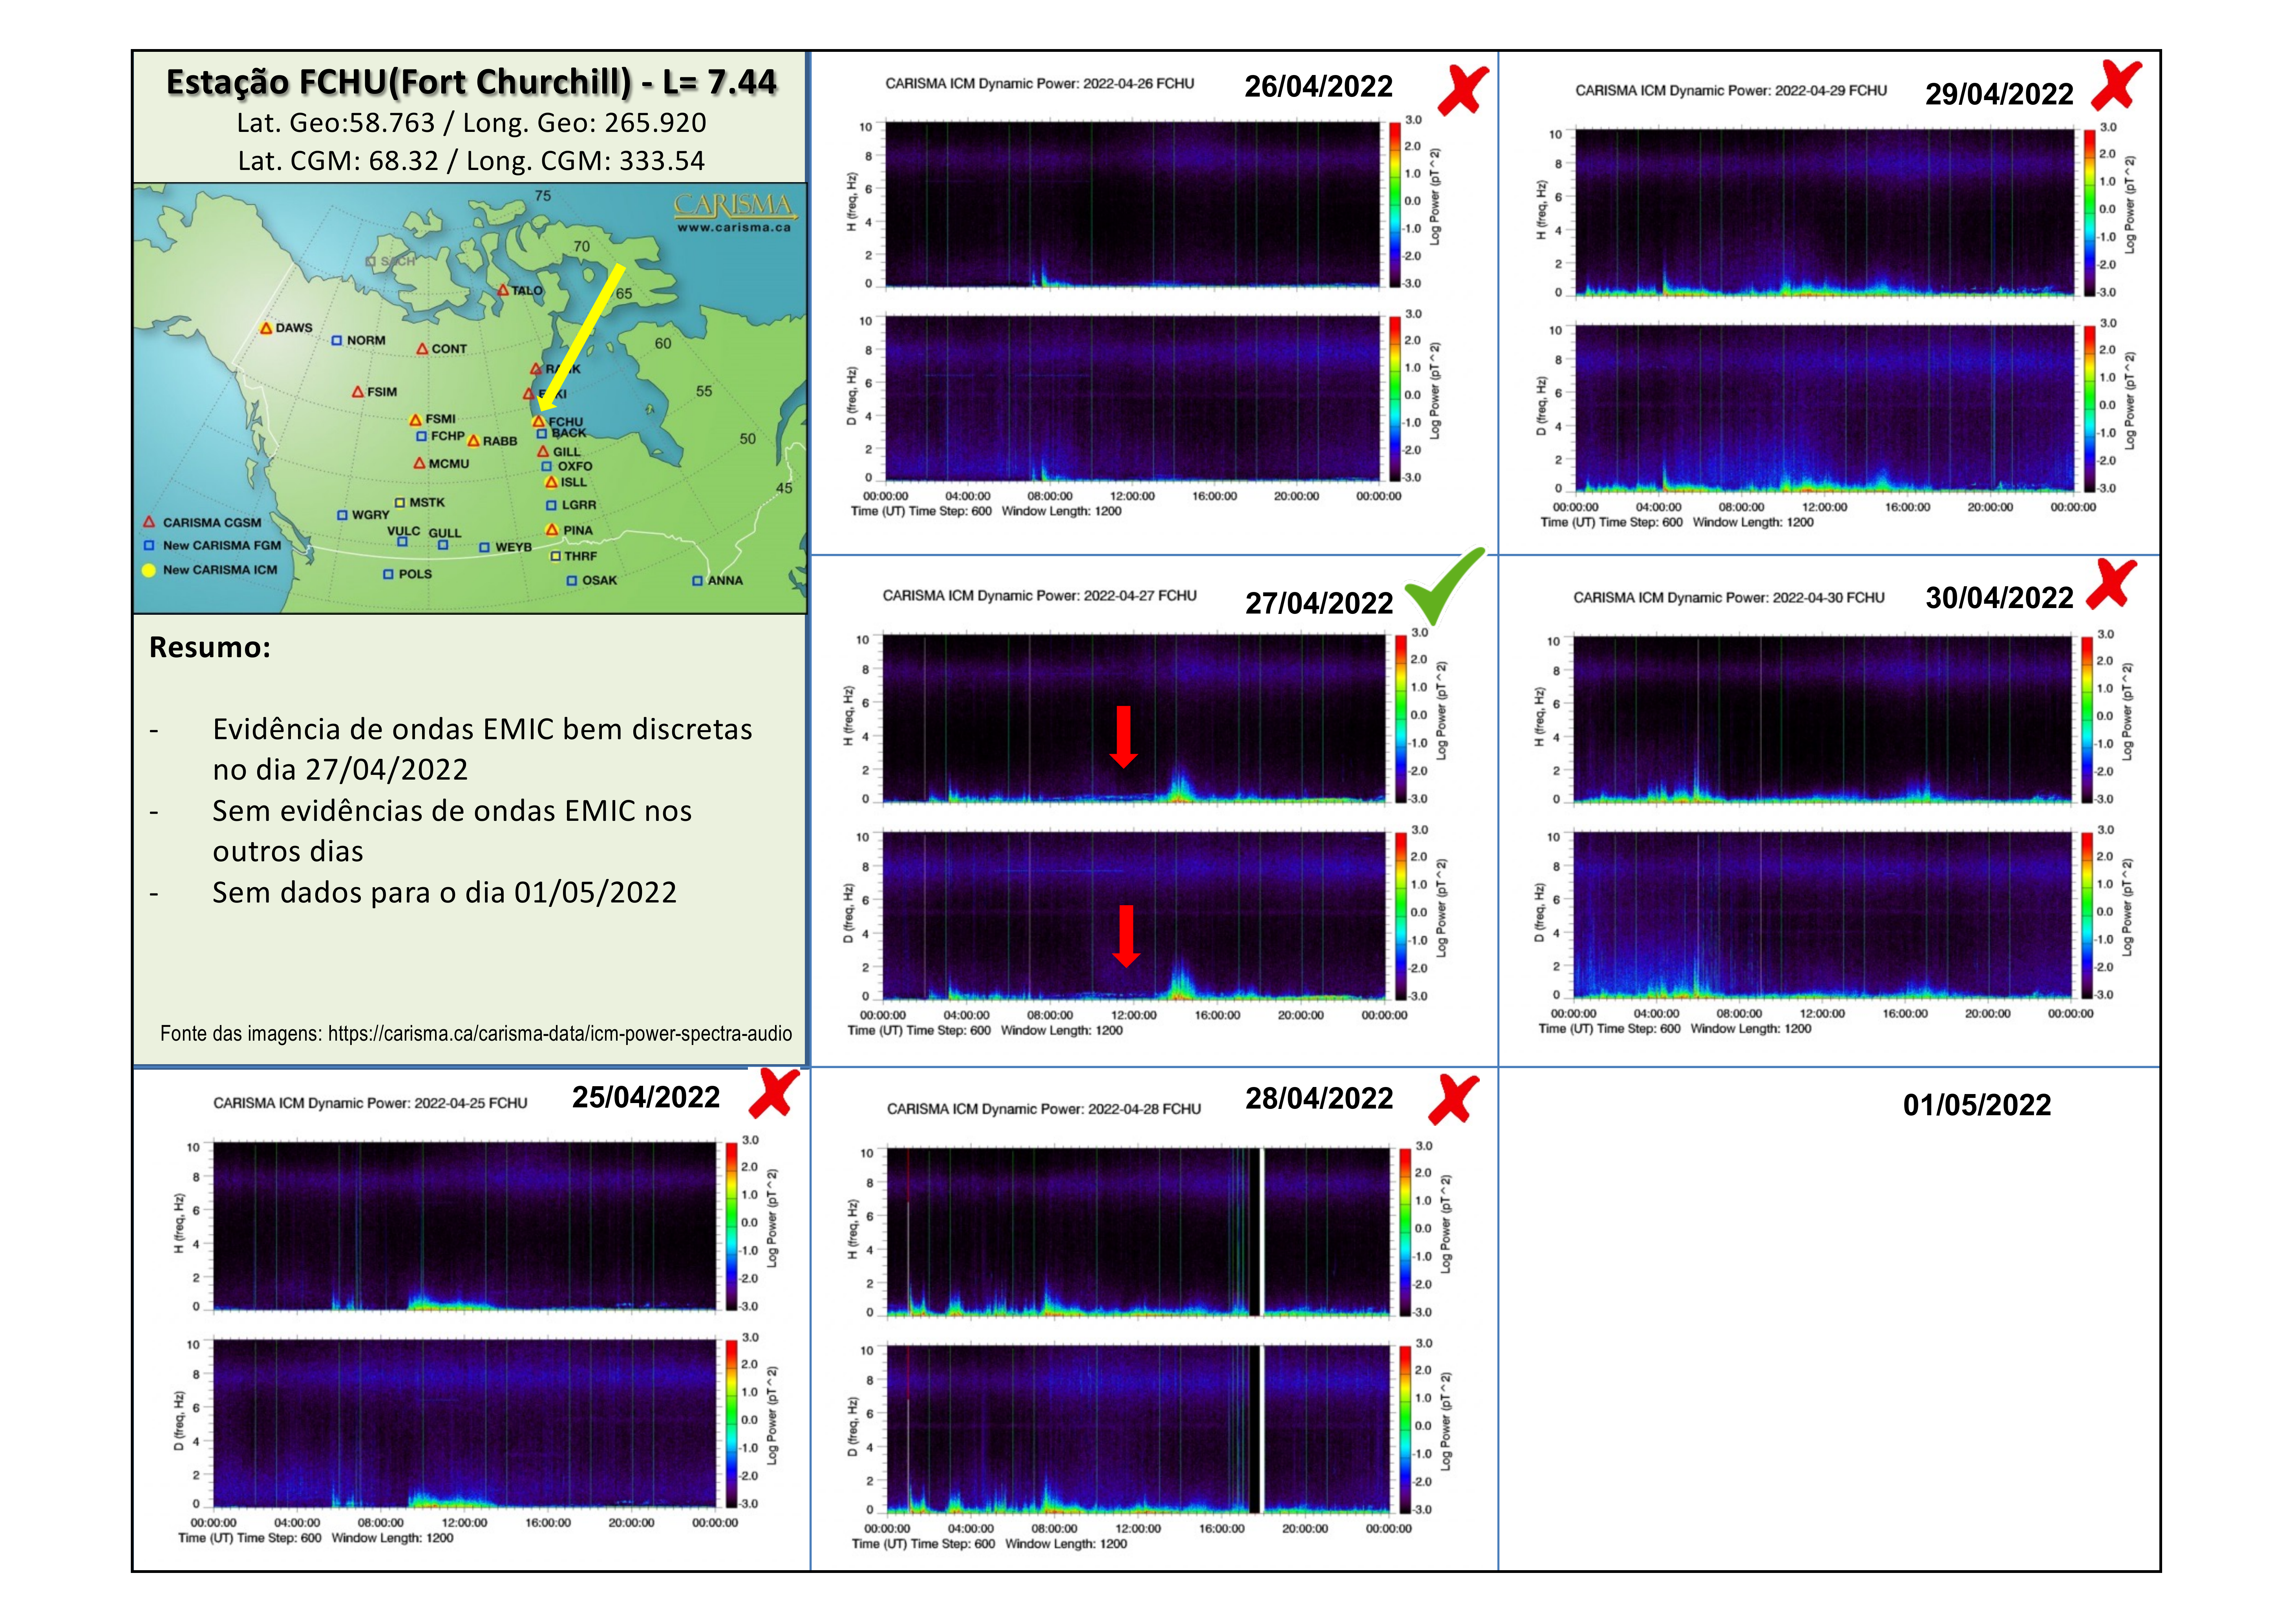
\includegraphics[width=14cm]{./figures//figureEMIC_1.png}

                        \end{figure}

                     \begin{figure}[H]
    
                        \centering
   
                             \includegraphics[width=14cm]{./figures//figureEMIC_2.png}

                        \end{figure}

                     \section{Geomagnetism} 
 \subsection{Responsible: Livia Riveiro Alves} 
 
\begin{figure}[H]
    
                        \centering
   
                             \includegraphics[width=14cm]{./figures//figureGeomag_0.png}

                        \end{figure}

                     \begin{figure}[H]
    
                        \centering
   
                             \includegraphics[width=14cm]{./figures//figureGeomag_1.png}

                        \end{figure}

                     \begin{figure}[H]
    
                        \centering
   
                             \includegraphics[width=14cm]{./figures//figureGeomag_2.png}

                        \end{figure}

                     \begin{figure}[H]
    
                        \centering
   
                             \includegraphics[width=14cm]{./figures//figureGeomag_3.png}

                        \end{figure}

                     \begin{figure}[H]
    
                        \centering
   
                             \includegraphics[width=14cm]{./figures//figureGeomag_4.png}

                        \end{figure}

                     \begin{figure}[H]
    
                        \centering
   
                             \includegraphics[width=14cm]{./figures//figureGeomag_5.png}

                        \end{figure}

                     \begin{figure}[H]
    
                        \centering
   
                             \includegraphics[width=14cm]{./figures//figureGeomag_6.png}

                        \end{figure}

                     \begin{figure}[H]
    
                        \centering
   
                             \includegraphics[width=14cm]{./figures//figureGeomag_7.png}

                        \end{figure}

                     \begin{figure}[H]
    
                        \centering
   
                             \includegraphics[width=14cm]{./figures//figureGeomag_8.png}

                        \end{figure}

                     \begin{itemize} 
\item In the week of 05/10 to 05/16, the following events related to geomagnetic activity stand out:
\item Data from the Embrace magnetometer network showed instabilities throughout the period, with some events highlighted:
\item The biggest disturbances in the H component were recorded on the 11th, 13th, and 14th of May.
\item Geomagnetic activity was unstable throughout the AE index, with the Dst index oscillating around zero. Highest Kp of the week was 3+
\item  The auroral activity was slightly intensified on the 13th, 14th and 15 thof May.
\end{itemize} 
\section{Ionosphere} 
 \subsection{Responsible: Laysa Resende} 
 
\textbf{Boa Vista: }

 \begin{itemize}
\item There were spread F during all days in this week.
\item The Es layers reached scale 3 on days 12 and 13.
\item There was partial blackout on day 10. 
\end{itemize}
\begin{figure}[H]
    \centering
    \includegraphics[width=14cm]{./figures//BoaVista.png}
\end{figure}

\textbf{Cachoeira Paulista:}

 \begin{itemize}
\item There were spread F on day 12.
\item The Es layers reached scale 3 on days 09, and 12. 
\end{itemize}
\begin{figure}[H]
    \centering
    \includegraphics[width=14cm]{./figures//CachoeiraPaulista.png}
\end{figure}

\textbf{São Luís: }

 \begin{itemize}
\item There were spread F during all days in this week.
\item The Es layers reached scale 5 on day 11. 
\item There was partial blackout on day 10. 
\end{itemize}
\begin{figure}[H]
    \centering
    \includegraphics[width=14cm]{./figures//SãoLuís.png}
\end{figure}

\section{Scintilation} 
 \subsection{Responsible: Siomel Savio Odriozola} 
 
In this report on the S4 scintillation index, data from SLMA in São Luiz/MA, STSN 
in Sinop/MG, UFBA in Bahía/BA and SJCE in São José dos Campos/SP are 
presented. The S4 index tracks the presence of irregularities in the ionosphere 
having a spatial scale ~ 360 m. 
The four analyzed stations did not present relevant values of the S4 index 
throughout the week. Figure 1 shows the values for SLMA(top panel) and 
SJCE(bottom panel) stations 

    \begin{figure}[H]
        \centering
        \includegraphics[width=14cm]{./figures/en_outfileScint_0.jpg}
    \end{figure} 
 

    

\end{document}